\section{General architecture}
The structure of the project can be best described as an implementation of the multitier architecture consisting of the Translation Memory Core, the User Space and the web application GUI, as can be seen in the figure \ref{projectStructure:layers}.

\begin{figure}[h]
\begin{center}
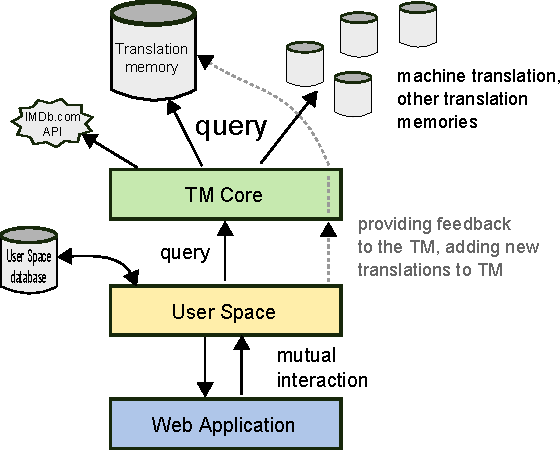
\includegraphics{figures/scheme.pdf}
\end{center}
\caption{Scheme of the application architecture.}\label{projectStructure:layers}
\end{figure}

The deepest level of the application is the Translation Memory Core which operates directly with the parallel chunks stored in database. It is implemented in Scala. It provides an interface for retrieving translation suggestions from multiple sources -- different ways of processing our own translation memory, publicly available translation memories or a machine translation output. It also assigns a score for each suggestion based on the retrieval parameters (typically the match score) and movie characteristics taken from the IMDb.com API.

The middle-ware layer is called the User Space (US). Its task is to interact with the translation memory itself and mirror all GUI operations on the server side. The User Space is implemented in Java. The TM Core is used only as a service which is queried for translation suggestions. The interaction with the GUI is much more complicated because each operation from GUI has to be reflected in the US. The US provides a permanent storage of users' work to make the whole application including the users data available from the Internet. Except this function, the US provides the TM suggestion for the GUI and keep them up to date (the TM is gradually improving, so after a week pause in work and a subtitle file, some better sentences in TM may occur).

GUI is written in Java, using GWT, which translates Java code into JavaScript and provides a framework for simple implementation of remote procedure calls (RPCs) through HTTP protocol, using POST requests. Server side of GUI layer displays the needed javascript and css code to user's browser, which, then, communicates with userspace through javascript AJAX calls through RPC, as described above. The GUI let the user log in, upload the subtitles, parses the subtitles to chunks, offer the user translations for every chunk and play the video of the chunks being translated.

Translation memory core and userspace are both parts of the same \texttt{.jar} file and are, therefore, run in the same java process. Userspace is running as a java servlet, because it is replying to RPC, which are implemented using HTTP post requests.

Server-side of GUI, which returns the HTML, CSS and JavaScript, is also in the same \texttt{.jar} file, together with needed GWT assets, and is run as a second servlet.

Both servlets are loaded using jetty webserver. Maven is used for building the application and retrieving dependencies, the Jenkins tool was used for continual building and testing of the project.

\section{Logical structure of work with TM}

In this section, the general structure of work with translation memory is described, from which a design of common classes is inferred, later used both in US, GUI and Core.

\subsection*{User}
Everyone, who logs into the system, is called \emph{user}. Each user of the TM, except its own setting, authentication data etc., can own multiple subtitle files which we call \emph{Documents}.

\subsection*{Document}
\emph{Document} is subtitle file, owned by a user. (This is not connected with files, that are used for building the corpus.) The documents contains information about \emph{media source} of the subtitle, and list of the subtitles \emph{chunks} which either have been already translated or are waiting for translation.

\subsection*{Media source}
\emph{Media source} is our name for movie or TV show episode.

\subsection*{Chunk}
Chunk is our name for a piece of text, that is getting translated. Chunk has a \emph{surface form} -- the text, being translated -- plus possible annotations. One of the annotations are named entities, but we also save newlines and dialogue marks ("-") as an annotation, so it doesn't go into database.

We talk more about the nature of subtitle files in the part \todo{???}???

\subsection*{Timed chunk}
Timed chunk is a chunk, that also have a time information and information about order, in which it appears in subtitle file.

\subsection*{Translation result}
The chunks are wrapped in to the \emph{Translation result} objects which contains the the timed chunk from the original subtitle file, a chunk produced by the user as a translation of the original chunk, a list of translation suggestions from translation memory \todo{Which are in fact WHAT? :)}which are in fact.


\begin{figure}[h]
\begin{center}
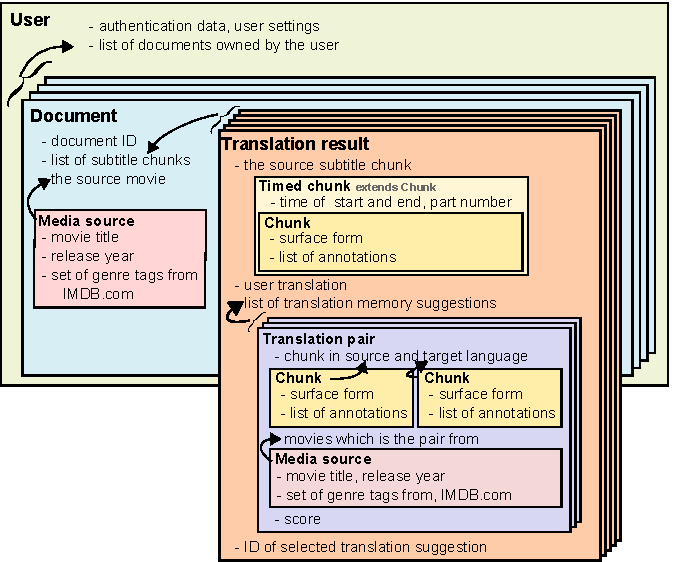
\includegraphics{figures/shared_classes.pdf}
\end{center}
\caption{Scheme of the application architecture.}\label{projectStructure:logical}
\end{figure}

All mentioned characteristics are common for both US and GUI. Because all parts of the project are Java based we can use a set of shared classes. Despite the limitations from to the fact, that the GWT implements only a subset of Java functionality, using a shared classes structure makes the whole project clearer. 

%If we look at the structure of a document being translated which is mirrored in the GUI and in the US, we can notice there together parts originating in different part of the projects.

\section{Sharing the implementation among the project}

Since we are using Google Web Toolkit (GWT), we can share java classes between GUI and server, as described in \todo{where}??.

However, as noted in GWT documentation \footnote{\url{https://developers.google.com/web-toolkit/doc/latest/DevGuideCodingBasicsCompatibility} and \url{https://developers.google.com/web-toolkit/doc/latest/RefJreEmulation}}, not all java classes are directly translatable to GWT. The main issues are:

\begin{itemize}
\item the shared classes cannot reference any class, that is not translatable to JavaScript through GWT (for example, any third-party libraries)
\item the shared classes can use only a subset of Java runtime library. In our case, main case of this was \texttt{java.util.regex}, which is not implemented in GWT; we had to use \texttt{com.google.gwt.regexp.shared} instead
\item serialization works differently in GWT. What this effectively meant for us is that, even when we use general \texttt{List} interface for some property, we cannot set it as subtype of \texttt{List} that is not implemented in GWT (more concretely -- we wanted to use \texttt{scala.collection.JavaConverters.AsJava[List]} for scala $\Leftrightarrow$ java conversion)
\end{itemize}

Therefore, shared classes could only use a subset of Java (generally, what is translatable with GWT to JavaScript is also translatable by java compiler to JVM bytecode, but not the other way around).
